\documentclass{article}

\usepackage[top=2cm, bottom=1.5cm, right=1.5cm, left=2cm]{geometry}
\usepackage{graphicx}
\usepackage{hyperref}

\author{Ana Larissa da Silva Dias \and Cassio Trindade Batista \and Edwin Jair Rueda \and Erick Modesto Campos}
\title{Disaster at St. Himark!\\VAST 2019 Mini Challenge 3}

\begin{document}
\maketitle

\begin{section}{Question}
\subsection{Characterize conditions across the city}
The earthquake appears to have started at 2~PM of the first day (April 6th), as
can be seen at the heatmap of Figure~\ref{fig:eq_start} (top). The heatmap is
divided by a time interval of one hour and by neighbourhood location. It was
generated by considering a list of keywords that were tweeted and are similar in 
meaning (synonyms) and are directly related to the word ``earthquake''. The list 
is: ``earthquake'', ``shake'', ``shudder'', ``vibrate'', ``wobble'', ``tremor'',
``tremble'', ``quaver'', ``quiver'', ``hazard'', ``disaster'', ``destruction'',
and ``rubble''.

To ensure the heatmap is providing a reliable information, a horizontal bar
chart was used. It counts isolated words and discards words such as adverbs,
pronouns, adjectives, articles and some nouns and verbs that were considered to
be useless such as ``anyone'', ``make'', ``know'', ``food'', ``hate'', etc. Then
the Porter Stemmer from the \texttt{nltk} package was used to clip the words by
its invariant parts (word root), and that root was further reduced to 4-chars
only. A heat-like colormap from blue to red was also included to enhance 
frequency distinction. 

\begin{figure}[!h]
    \centering
    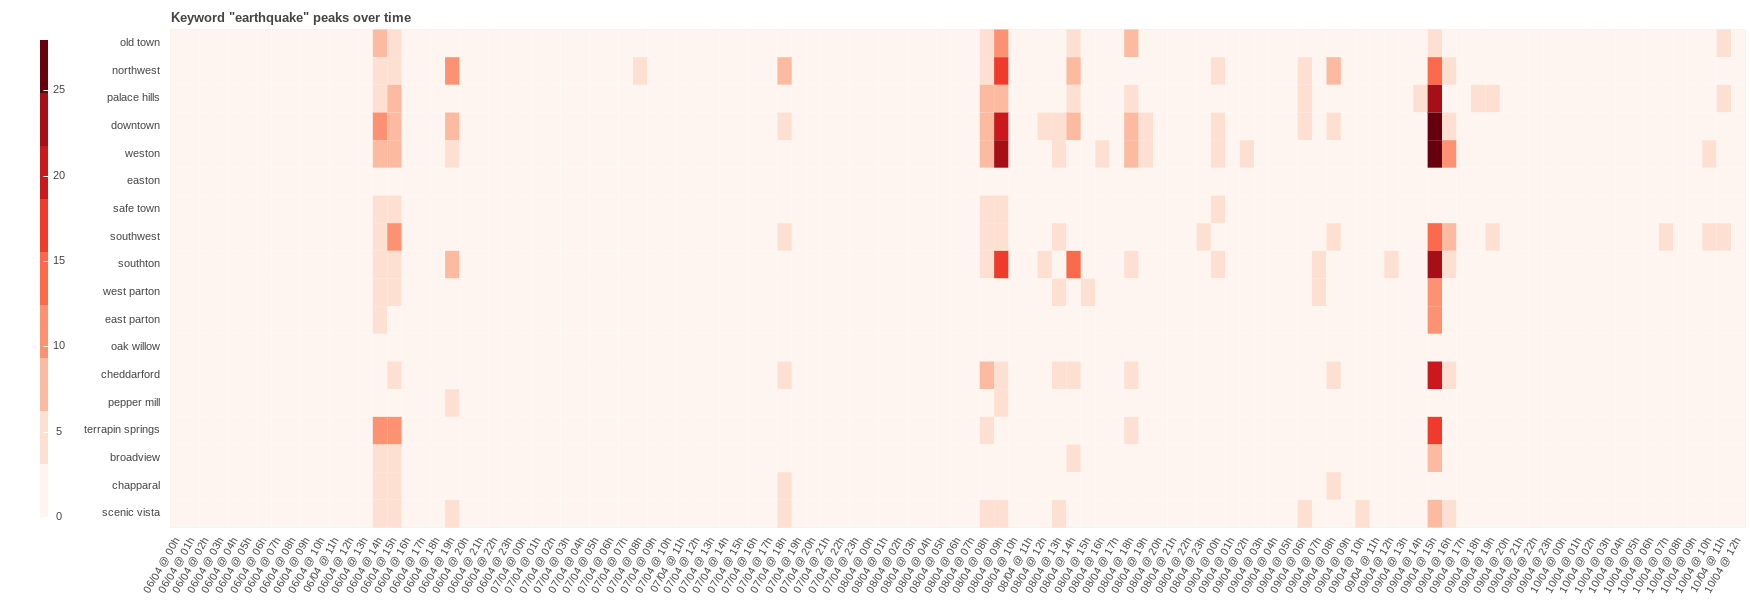
\includegraphics[width=1.00\textwidth]{figs/earthquake_start_heat.png}\\[12pt]
    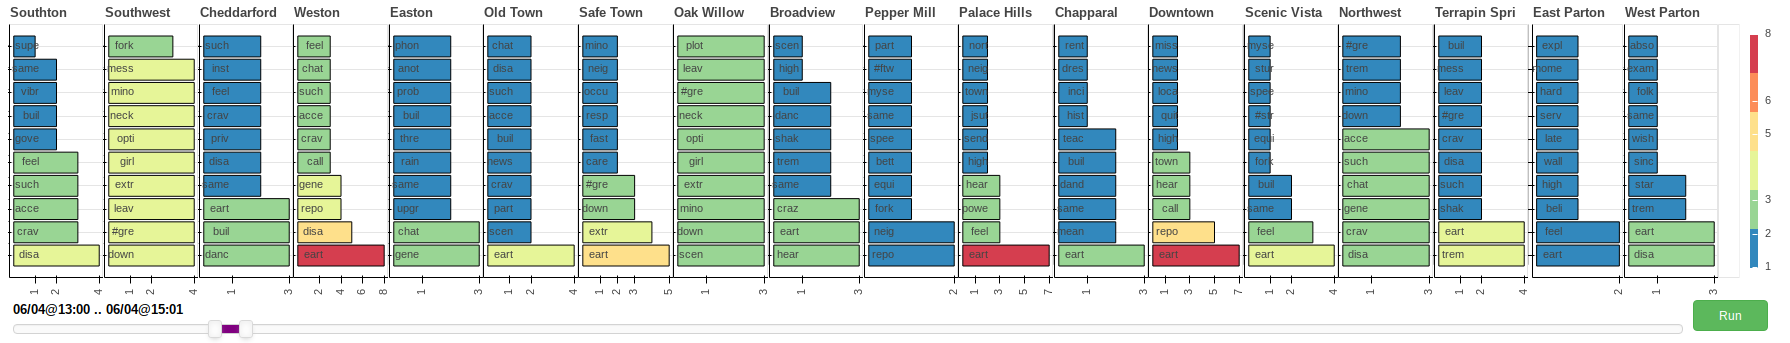
\includegraphics[width=1.00\textwidth]{figs/earthquake_start_hbar.png}
    \caption{Earthquake start}
    \label{fig:eq_start}
\end{figure}

\subsection{How resources should be allocated 5h after the earthquake?}
Figure~\ref{fig:eq_cond_5h} shows the heatmap per keyword in a five-hour-time 
interval from 1:00~PM to 6:59~PM. The top shows 3 blank graphs for the keywords
``building'', ``medical'', and ``road'', which means these resources do not 
appear to be requested by any neighbourhood. On the other hand, the 3 graphs at
the bottom show the number of mentions for keywords related to 
``sewer and water'', ``power'', and ``rain''. 
    
\begin{figure}[!h]
    \centering
    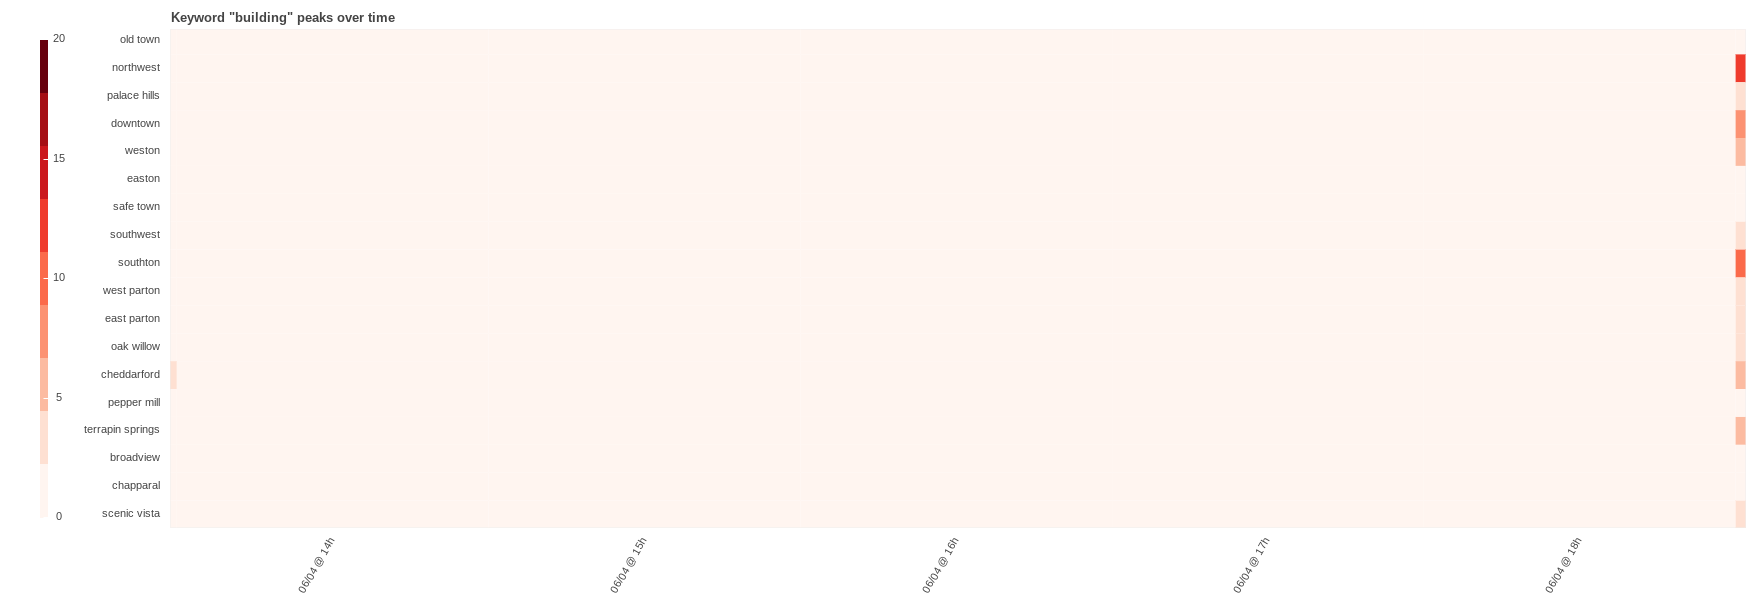
\includegraphics[width=0.30\textwidth]{figs/cond_5h/cond_5h_build.png}
    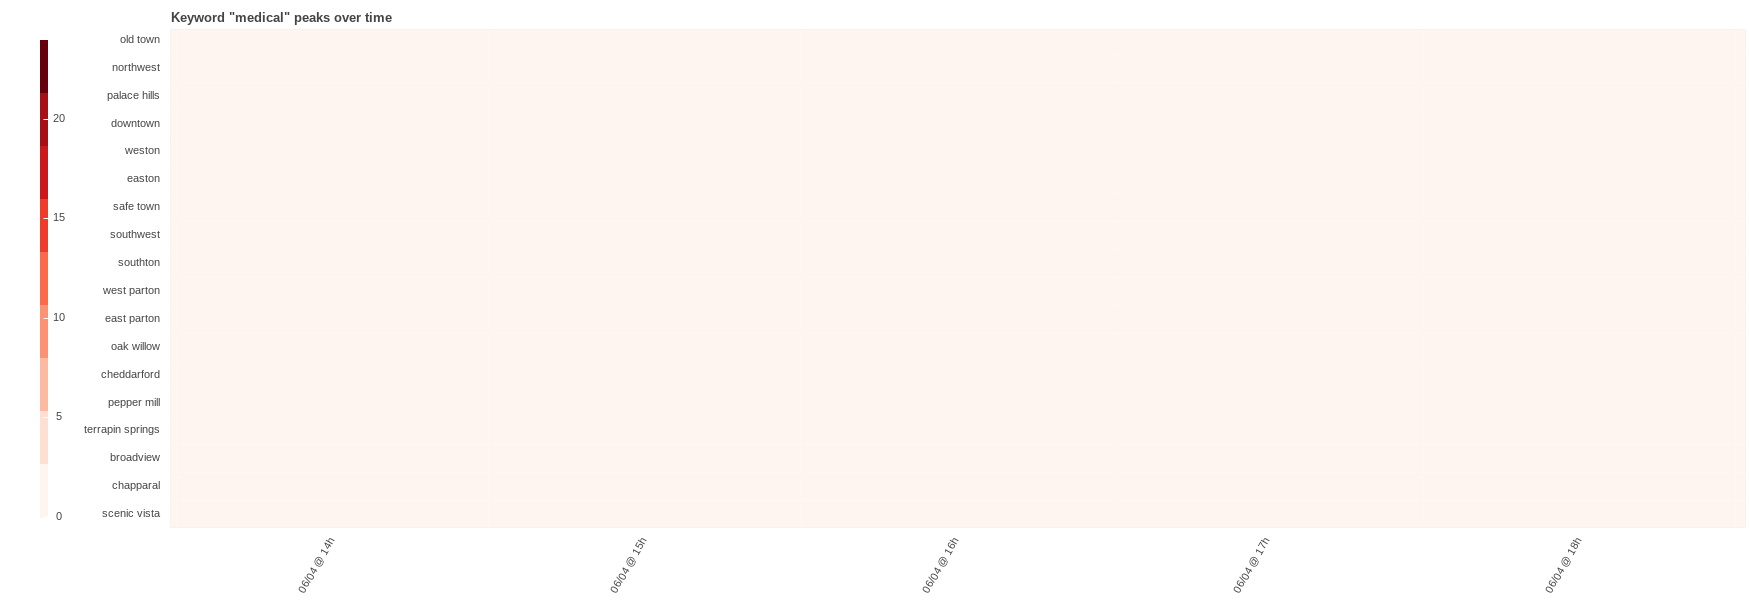
\includegraphics[width=0.30\textwidth]{figs/cond_5h/cond_5h_medical.png}
    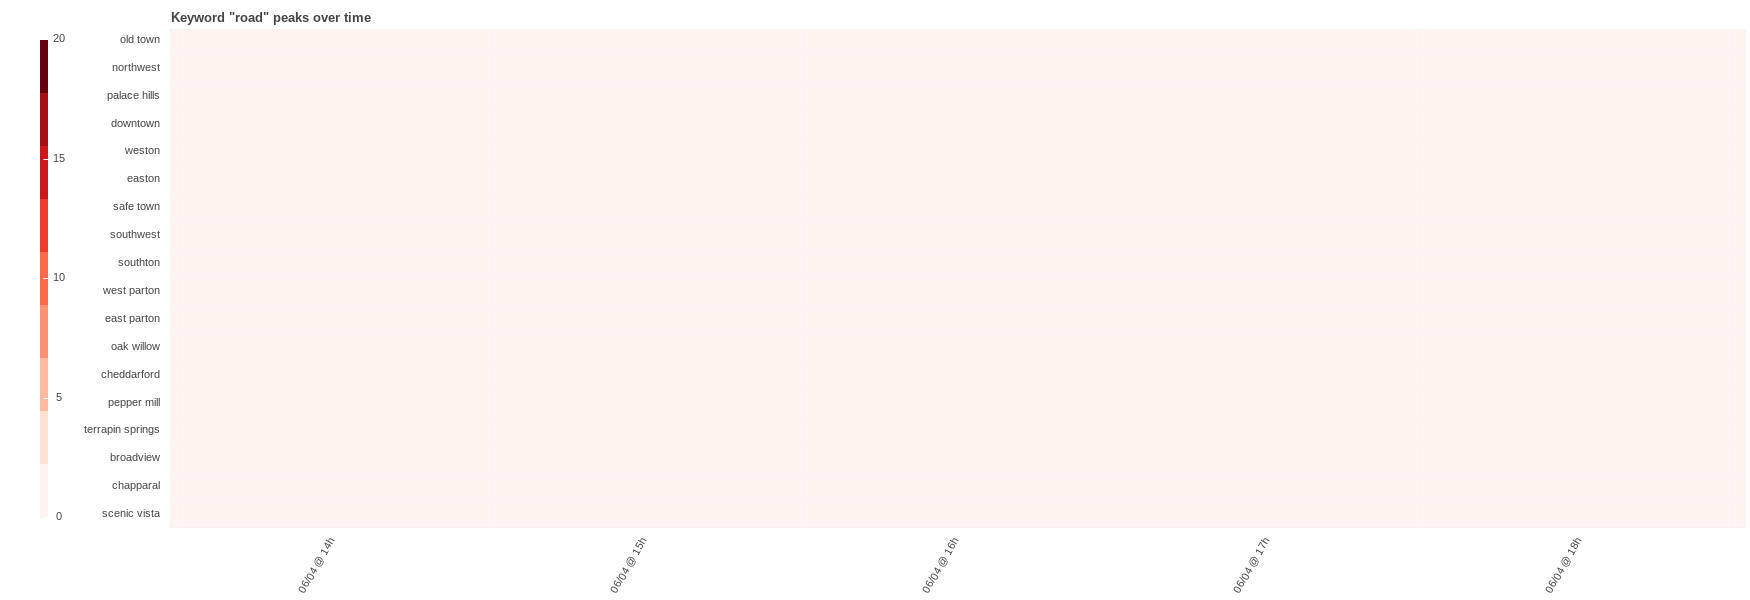
\includegraphics[width=0.30\textwidth]{figs/cond_5h/cond_5h_road.png}\\
    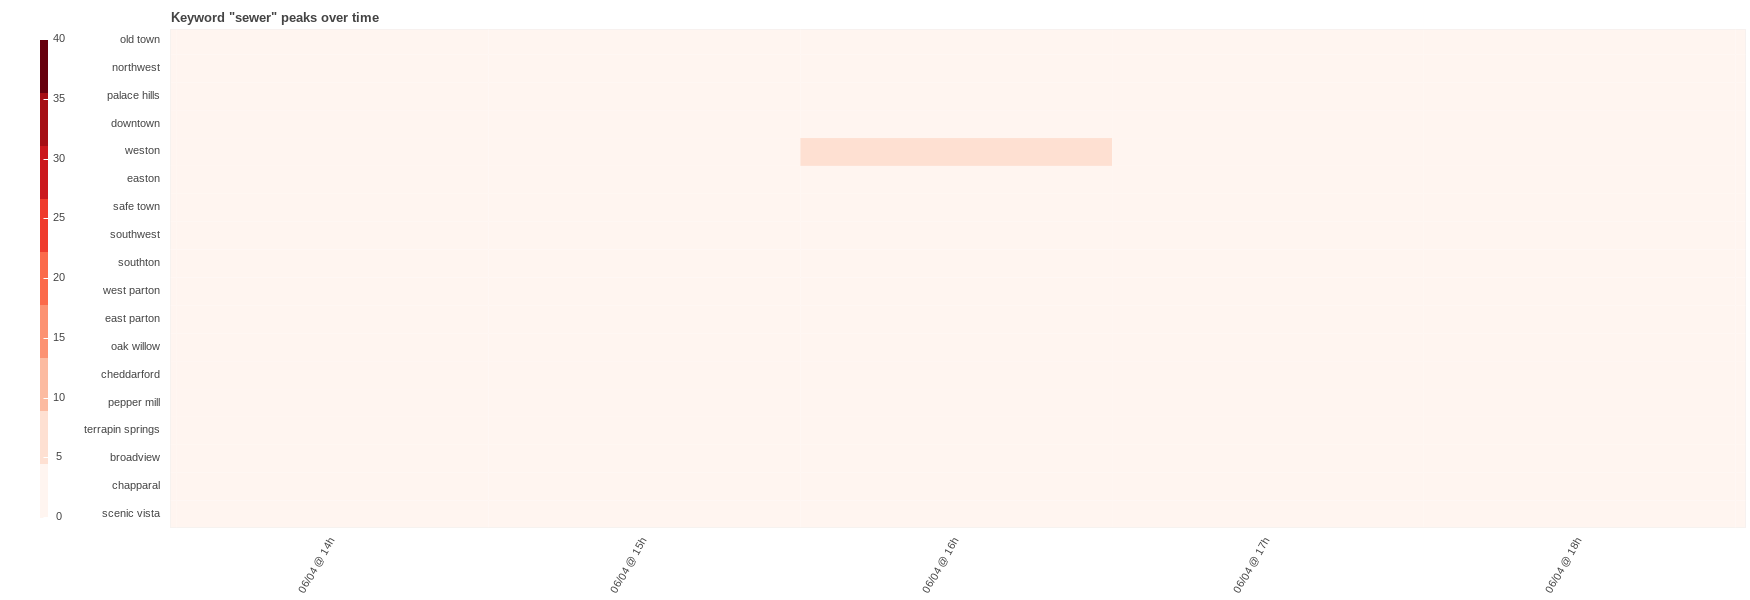
\includegraphics[width=0.30\textwidth]{figs/cond_5h/cond_5h_sewer.png}
    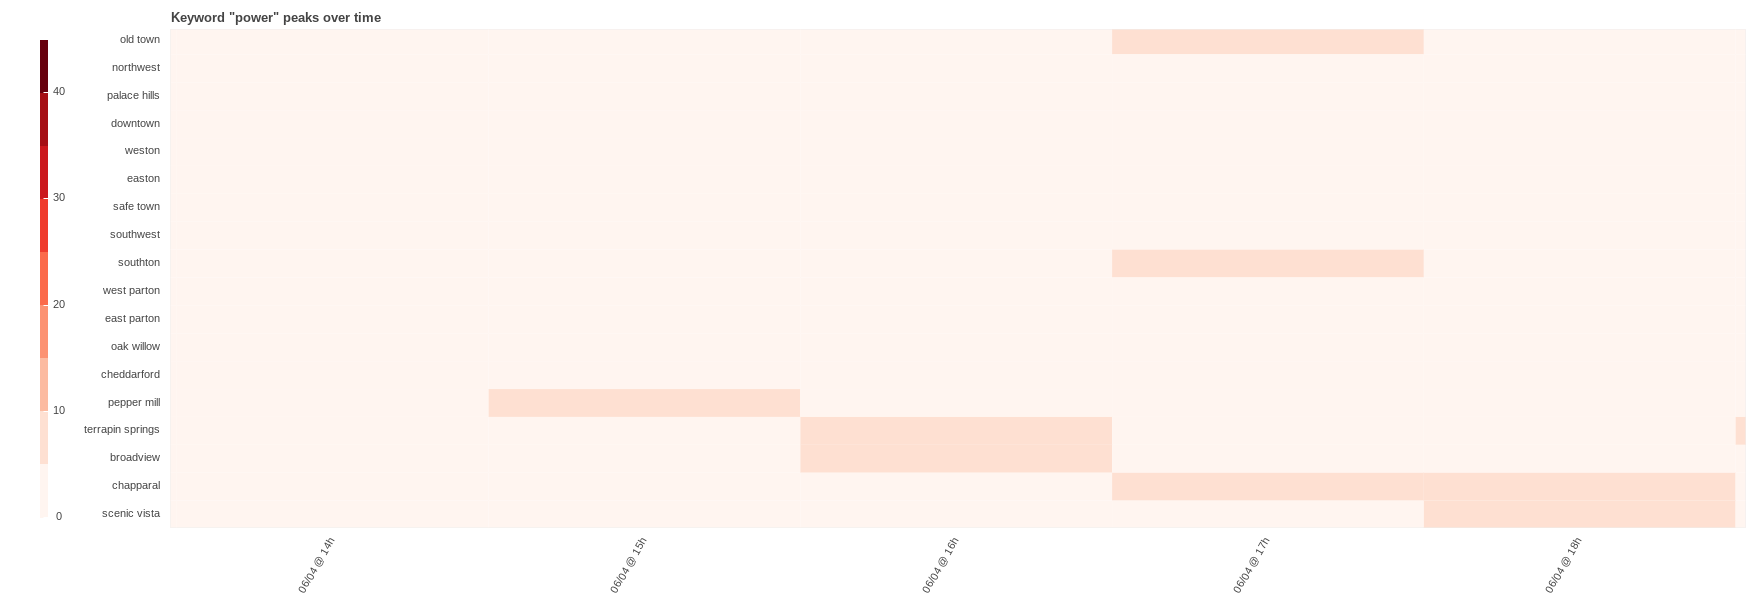
\includegraphics[width=0.30\textwidth]{figs/cond_5h/cond_5h_power.png}
    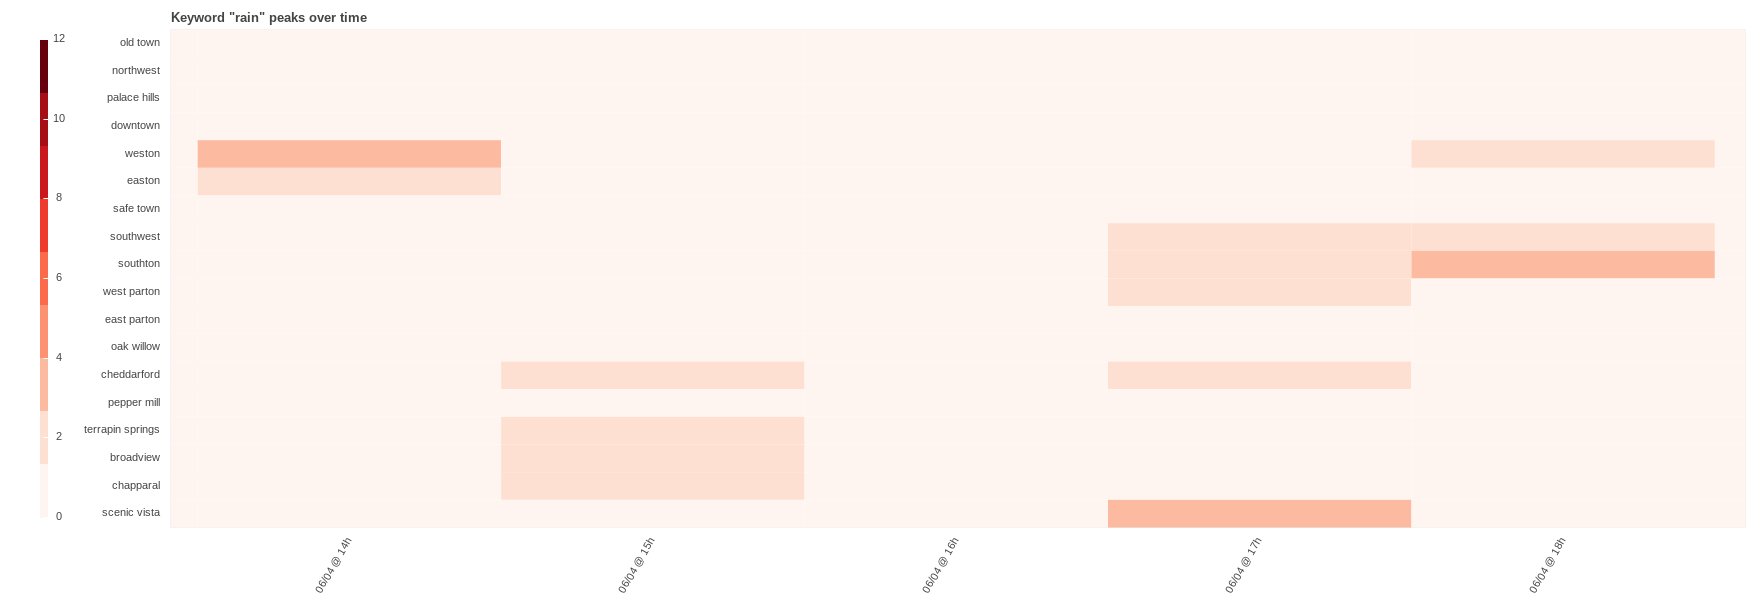
\includegraphics[width=0.30\textwidth]{figs/cond_5h/cond_5h_rain.png}
    \caption{Earthquake conditions after 5h}
    \label{fig:eq_cond_5h}
\end{figure}

Suggestions for crew allocation is detailed as follows: 

\begin{itemize}
    \item \emph{Sewer and water:} A crew must be sent only to Weston between 
    4:00~PM and 4:59~PM.
    \smallskip 
    \item \emph{Power}: Issues have occurred in Pepper Mill, \textbf{Terrapin
    Springs}, \textbf{Broadview}, Chapparal, \textbf{Southton}, \textbf{Old 
    Town} and Scenic Vista, but we'll consider only the locations 
    highlighted in bold because they have hospitals.
    \begin{itemize}
        \item A crew must be sent to Terrapin Springs between 3:00~PM and
        3:59~PM. Broadview also has a power demand at this time interval but the
        tweet frequency is much lower considering the five-hour period.
        \item Two crews must be sent to Old Town and Southton between 4:00~PM 
        and 4:59~PM.
        \item Lastly, the crew from Terrapin Springs can be reallocated to
        Chapparal between 5:00~PM and 5:59~PM. Although Chapparal does not have
        hospitals, it has been nearly two hours with electrical issues.
    \end{itemize}
    \item \emph{Rescue, sewer and water}: A crew must be sent to Southton only
    because there have been small issues in Weston, Southton and Downtown, and
    therefore Southton is geographically in the middle of such neighbourhoods.
\end{itemize}

\subsection{How resources should be allocated 30h after the earthquake?}
\end{section}


\end{document}
